\section{Architekturentwurf}

In diesem Kapitel wird der Architekturentwurf der BC Middleware mit Fokus auf die Austauschbarkeit der Backend-Implementierung beschrieben. Der Entwurf orientiert sich an etablierten Architekturprinzipien \citep{bass2021, starke2020} und berücksichtigt die spezifischen Anforderungen aus Kapitel~3.

\subsection{Gesamtarchitektur}

Die Middleware folgt einer Schichtenarchitektur mit klarer Trennung der Verantwortlichkeiten \citep{fowler2002}. In Abbildung~\ref{fig:architektur} werden die fünf Schichten und ihre Beziehungen dargestellt:

\begin{figure}[H]
\centering
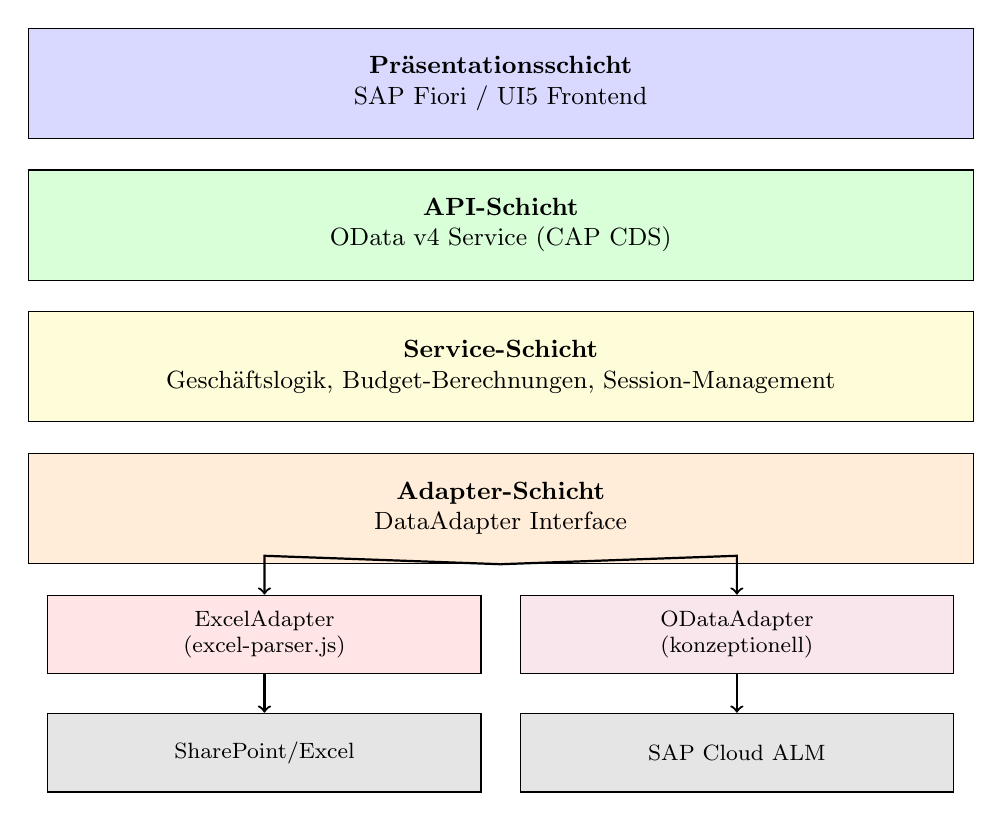
\begin{tikzpicture}[
    layer/.style={rectangle, draw, minimum width=12cm, minimum height=1.4cm, align=center, font=\small},
    sublayer/.style={rectangle, draw, minimum width=5.5cm, minimum height=1cm, align=center, font=\footnotesize}
]
    % Schichten
    \node[layer, fill=blue!15] (pres) at (0,6) {\textbf{Präsentationsschicht}\\SAP Fiori / UI5 Frontend};
    \node[layer, fill=green!15] (api) at (0,4.2) {\textbf{API-Schicht}\\OData v4 Service (CAP CDS)};
    \node[layer, fill=yellow!15] (service) at (0,2.4) {\textbf{Service-Schicht}\\Geschäftslogik, Budget-Berechnungen, Session-Management};
    \node[layer, fill=orange!15] (adapter) at (0,0.6) {\textbf{Adapter-Schicht}\\DataAdapter Interface};

    % Adapter-Implementierungen
    \node[sublayer, fill=red!10] (excel) at (-3,-1) {ExcelAdapter\\(excel-parser.js)};
    \node[sublayer, fill=purple!10] (odata) at (3,-1) {ODataAdapter\\(konzeptionell)};

    % Datenquellen
    \node[sublayer, fill=gray!20] (sp) at (-3,-2.5) {SharePoint/Excel};
    \node[sublayer, fill=gray!20] (calm) at (3,-2.5) {SAP Cloud ALM};

    % Verbindungen
    \draw[->, thick] (adapter.south) -- (-3,0) -- (excel.north);
    \draw[->, thick] (adapter.south) -- (3,0) -- (odata.north);
    \draw[->, thick] (excel.south) -- (sp.north);
    \draw[->, thick] (odata.south) -- (calm.north);
\end{tikzpicture}
\caption{Gesamtarchitektur der BC Middleware}
\label{fig:architektur}
\end{figure}

Die oberste Schicht bildet die Präsentationsschicht mit dem Fiori Frontend, das nicht Teil dieser Arbeit ist. Darunter liegt die API-Schicht, die einen \gls{odata} v4 Service über SAP \gls{cap} bereitstellt. Die Service-Schicht kapselt die Geschäftslogik und Berechnungen, während die Adapter-Schicht den konkreten Datenzugriff über den Excel-Parser oder einen OData-Connector realisiert. Die unterste Ebene bildet die Datenschicht mit SharePoint/Excel oder \gls{calm} Services als Datenquellen.

\subsection{Schichtenmodell}

Im Folgenden werden die einzelnen Schichten der Architektur (vgl. Abbildung~\ref{fig:architektur}) detailliert beschrieben.

\subsubsection{Präsentationsschicht}

Die Präsentationsschicht umfasst das SAP Fiori Frontend, das von anderen Studierenden im Rahmen separater Arbeiten entwickelt wird. Sie ist bewusst nicht Bestandteil dieser Arbeit, stellt jedoch eine zentrale Randbedingung dar: Die Middleware muss eine \gls{odata} v4-konforme \gls{api} bereitstellen, da SAP Fiori diese als Standard für die Datenkommunikation voraussetzt \citep{sap2024cap}. Sämtliche Entwurfsentscheidungen der darunterliegenden Schichten orientieren sich an dieser Anforderung.

\subsubsection{API-Schicht}

Die API-Schicht wird mit SAP \gls{cap} implementiert und stellt eine \gls{odata} v4-konforme Schnittstelle bereit. Die Service-Definition erfolgt deklarativ in \gls{cds}, wobei die Annotation \texttt{@cds.persistence.skip} eine zentrale Rolle spielt: Sie kennzeichnet Entitäten, die nicht in einer Datenbank persistiert werden, sondern zur Laufzeit aus anderen Quellen generiert werden. Dadurch übernimmt \gls{cap} automatisch die Bereitstellung von OData-Funktionalitäten wie Filterung (\texttt{\$filter}), Paginierung (\texttt{\$top}/\texttt{\$skip}) und Sortierung (\texttt{\$orderby}), ohne dass diese manuell implementiert werden müssen. Die API exponiert insgesamt acht lesbare Entitäten (darunter \texttt{BudgetOverview} und \texttt{UserStories}), zwei Funktionen (\texttt{getProjects}, \texttt{getSessionInfo}) sowie vier Actions für Session-Management und \gls{psp}-Zuordnungen.

\subsubsection{Service-Schicht}

Die Service-Schicht bildet den Kern der Middleware und kapselt die gesamte Geschäftslogik. Sie ist in SAP \gls{cap} als \texttt{ApplicationService} implementiert und folgt dem ereignisgesteuerten Handler-Modell des Frameworks: Für jede Entität wird ein \texttt{on('READ')}-Handler registriert, der die Daten zur Laufzeit aus der Adapter-Schicht lädt und aufbereitet.

Die Schicht gliedert sich intern in drei Verantwortungsbereiche. Der erste Bereich umfasst die Budget-Berechnung, die in ein eigenständiges Modul (\texttt{budget-calculations.js}) ausgelagert wurde. Dieses Modul aggregiert die vier Metriken Budget, Actual, \gls{etc} und \gls{eac} sowohl pro Team als auch pro \gls{psp}-Element und ist bewusst frei von Abhängigkeiten zur Datenquelle gehalten, was eine isolierte Testbarkeit ermöglicht. Der zweite Bereich ist das Session-Management, das sicherstellt, dass jeder Client über einen \texttt{x-session-id}-Header einem Projekt zugeordnet wird. Sessions werden im Arbeitsspeicher gehalten und nach acht Stunden automatisch invalidiert. Der dritte Bereich umfasst die Validierungslogik, insbesondere die Prüfung auf Team-Mismatches bei \gls{psp}-Zuordnungen, bei denen das Team der User Story vom Team des \gls{psp}-Elements abweicht.

\subsubsection{Adapter-Schicht}

Die Adapter-Schicht abstrahiert den Zugriff auf die Datenquellen und stellt der Service-Schicht ein einheitliches Datenmodell zur Verfügung -- unabhängig davon, ob die Daten aus einer Excel-Datei oder einem OData-Service stammen. Die Service-Schicht ruft ausschließlich Methoden der Adapter-Schnittstelle auf (etwa \texttt{loadTeams()}, \texttt{loadUserStories()} oder \texttt{savePSPAssignment()}) und hat keine Kenntnis über die konkrete Datenquelle. Dieses Prinzip der Umkehrung der Abhängigkeit (\textit{Dependency Inversion}) ist ein Kernelement austauschbarer Architekturen \citep{gamma1994}. Die Adapter-Schicht wird in Abschnitt~4.3 im Detail beschrieben.

\subsubsection{Datenschicht}

Die Datenschicht bezeichnet die externen Datenquellen selbst. Im aktuellen Zustand ist dies eine \texttt{Budgetcontrolling.xlsx} auf dem lokalen Dateisystem (bzw. perspektivisch auf SharePoint), die über Power Query mit Daten aus SAP \gls{calm} befüllt wird. Bei einem späteren Backend-Wechsel würde diese Schicht durch die OData-Services von SAP \gls{calm} ersetzt, ohne dass die darüberliegenden Schichten angepasst werden müssen.

\subsection{Adapter-Pattern für Backend-Austauschbarkeit}

Der zentrale Entwurfsgedanke besteht in der Austauschbarkeit des Backends. Die Adapter-Schicht definiert eine einheitliche Schnittstelle, welche von beiden Backend-Implementierungen erfüllt wird \citep{gamma1994}. In Abbildung~\ref{fig:adapter-detail} ist das Klassendiagramm dargestellt.

\begin{figure}[H]
\centering
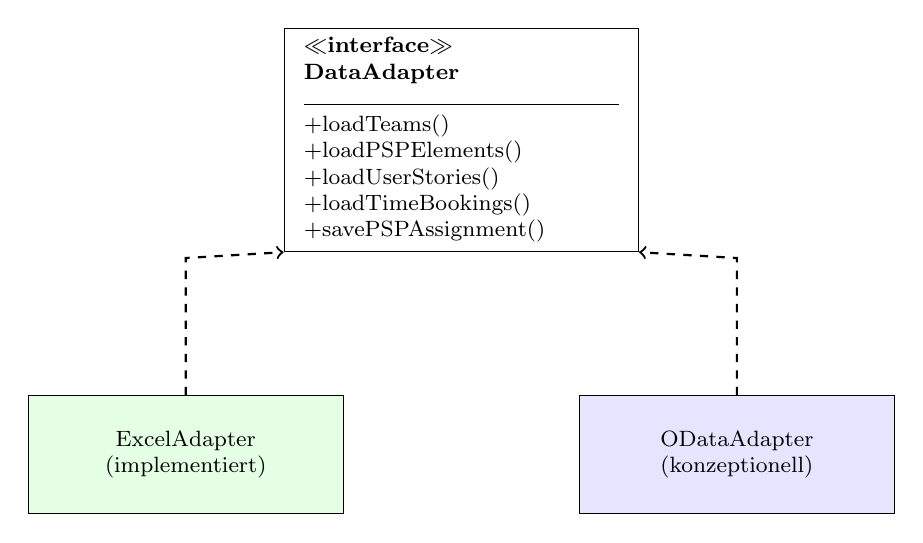
\begin{tikzpicture}[
    interface/.style={rectangle, draw, minimum width=4.5cm, minimum height=2.5cm, align=left, font=\footnotesize},
    class/.style={rectangle, draw, minimum width=4cm, minimum height=1.5cm, align=center, font=\footnotesize}
]
    % Interface
    \node[interface] (iface) at (0,0) {
        \textbf{$\ll$interface$\gg$}\\
        \textbf{DataAdapter}\\
        \rule{4cm}{0.4pt}\\
        +loadTeams()\\
        +loadPSPElements()\\
        +loadUserStories()\\
        +loadTimeBookings()\\
        +savePSPAssignment()
    };

    % Implementierungen
    \node[class, fill=green!10] (excel) at (-3.5,-4) {ExcelAdapter\\(implementiert)};
    \node[class, fill=blue!10] (odata) at (3.5,-4) {ODataAdapter\\(konzeptionell)};

    % Vererbungspfeile
    \draw[->, thick, dashed] (excel.north) -- (-3.5,-1.5) -- (iface.south west);
    \draw[->, thick, dashed] (odata.north) -- (3.5,-1.5) -- (iface.south east);
\end{tikzpicture}
\caption{DataAdapter Interface und Implementierungen}
\label{fig:adapter-detail}
\end{figure}

\begin{lstlisting}[caption={Adapter-Interface (konzeptionell)}, label={lst:adapter-interface}]
interface DataAdapter {
    loadTeams(): Team[]
    loadPSPElements(): PSPElement[]
    loadUserStories(): UserStory[]
    loadTimeBookings(): TimeBooking[]
    loadPSPAssignments(): PSPAssignment[]

    savePSPAssignment(assignment): void
    updatePSPAssignment(assignment): void
    deletePSPAssignment(key): void
}
\end{lstlisting}

\subsubsection{Excel-Adapter}

Der Excel-Adapter ist die aktuell implementierte Variante des DataAdapter-Interfaces. Er liest sämtliche Daten aus einer einzigen \texttt{Budgetcontrolling.xlsx}, die mehrere Sheets mit unterschiedlichen Strukturen enthält (vgl. Tabelle~\ref{tab:excel-sheets} in Kapitel~3). Die zentrale Herausforderung besteht darin, diese heterogenen Sheet-Formate -- tabellarische Stammdaten, SAP-Listenexporte mit spezieller Spaltenstruktur und manuell gepflegte Zuordnungstabellen -- auf ein einheitliches Datenmodell abzubilden.

Der Adapter übernimmt dabei drei Aufgaben. Erstens das Parsen der verschiedenen Sheets: Jedes Sheet erfordert eine individuelle Parsing-Logik, da sich Spaltenbezeichnungen, Datentypen und Startzeilen unterscheiden. Insbesondere das CADO-Sheet mit den Zeitbuchungen weicht vom Standardformat ab, da es als SAP-Listenexport ein spezielles Spaltenlayout und das deutsche Zahlenformat verwendet. Zweitens das Mapping auf das einheitliche Datenmodell: Die geparsten Rohdaten werden in die \gls{cds}-Entitäten überführt, sodass die Service-Schicht keine Kenntnis über die Excel-Struktur benötigt. Drittens der Write-Back für \gls{psp}-Zuordnungen: Neue, geänderte oder gelöschte Zuordnungen werden direkt in das Sheet \enquote{1. PSP-Zuordnung} geschrieben, wobei die übrigen Sheets unverändert bleiben.

Ein besonderer Aspekt ist der PSP-Override-Mechanismus (vgl. Abschnitt~4.6): Manuelle Zuordnungen aus dem \enquote{1. PSP-Zuordnung}-Sheet überschreiben die ursprünglichen PSP-Zuordnungen aus \texttt{qry\_CALM\_Data}, sodass Änderungen über die \gls{api} sofort wirksam werden, ohne dass die Power-Query-Verbindung in Excel aktualisiert werden muss.

\subsubsection{OData-Adapter (konzeptionell)}

Der OData-Adapter ist die perspektivische Alternative zum Excel-Adapter und würde Daten direkt von den OData-Services des SAP \gls{calm} abrufen. Er ist im Rahmen dieser Arbeit nicht implementiert, jedoch so konzipiert, dass er das gleiche DataAdapter-Interface erfüllt und somit den Excel-Adapter ohne Änderungen an der Service-Schicht ersetzen kann.

Anstatt eine lokale Excel-Datei zu parsen, würde der OData-Adapter HTTP-Requests an die \gls{calm}-\gls{api} senden, um User Stories, Zeitbuchungen und Projektstrukturen abzurufen. Die Authentifizierung erfolgt über den OAuth 2.0 Client Credentials Flow, da die Middleware als Server-zu-Server-Anwendung ohne Benutzerinteraktion agiert. Das Mapping der \gls{calm}-Datenstrukturen auf das interne Datenmodell der Middleware übernimmt der Adapter analog zum Excel-Adapter, sodass die Budget-Berechnungslogik identisch bleibt. Der wesentliche Unterschied liegt darin, dass Echtzeitdaten zur Verfügung stünden, da keine manuelle Aktualisierung der Excel-Power-Query mehr erforderlich wäre. Der geschätzte Implementierungsaufwand für diesen Adapter wird in Kapitel~6 evaluiert.

\subsection{Session-Management}

Die Middleware unterstützt mehrere Projekte. Über ein Session-Management wird sichergestellt, dass alle Requests eines Benutzers auf das gleiche Projekt zugreifen.

\begin{lstlisting}[caption={Session-Flow}, label={lst:session-flow}]
1. GET  /api/budget/getProjects()
   -> ["Projekt_1", "Projekt_2"]

2. POST /api/budget/startSession { "project": "Projekt_1" }
   -> { sessionId: "abc123...", project: "Projekt_1" }

3. GET  /api/budget/BudgetOverview
   Header: x-session-id: abc123...
   -> Budget-Daten fuer Projekt_1
\end{lstlisting}

\subsection{Datenmodell}

Das Datenmodell orientiert sich an den Excel-Strukturen und wird in \gls{cds} definiert. Es folgt den Prinzipien des Domain-Driven Design \citep{evans2003, vernon2013} und bildet die Domänenkonzepte des Budget-Controllings ab. Abbildung~\ref{fig:er-diagramm} zeigt die Beziehungen zwischen den Entitäten.

\begin{figure}[H]
\centering
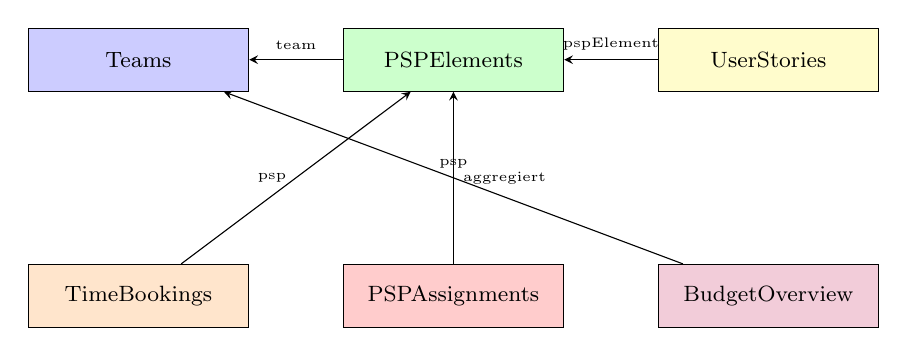
\begin{tikzpicture}[
    entity/.style={rectangle, draw, minimum width=2.8cm, minimum height=0.8cm, align=center, font=\footnotesize},
    arrow/.style={->, >=stealth}
]
    % Entitäten
    \node[entity, fill=blue!20] (team) at (0,3) {Teams};
    \node[entity, fill=green!20] (psp) at (4,3) {PSPElements};
    \node[entity, fill=yellow!20] (us) at (8,3) {UserStories};
    \node[entity, fill=orange!20] (tb) at (0,0) {TimeBookings};
    \node[entity, fill=red!20] (pa) at (4,0) {PSPAssignments};
    \node[entity, fill=purple!20] (bo) at (8,0) {BudgetOverview};

    % Beziehungen
    \draw[arrow] (psp) -- node[above, font=\tiny] {team} (team);
    \draw[arrow] (us) -- node[above, font=\tiny] {pspElement} (psp);
    \draw[arrow] (tb) -- node[left, font=\tiny] {psp} (psp);
    \draw[arrow] (pa) -- node[above, font=\tiny] {psp} (psp);
    \draw[arrow] (bo) -- node[right, font=\tiny] {aggregiert} (team);
\end{tikzpicture}
\caption{Vereinfachtes ER-Diagramm der Entitäten}
\label{fig:er-diagramm}
\end{figure}

\subsubsection{Entitäten}

\begin{table}[H]
\centering
\caption{Übersicht der Entitäten}
\label{tab:entities}
\begin{tabularx}{\textwidth}{l>{\raggedright\arraybackslash}X}
\toprule
\textbf{Entität} & \textbf{Beschreibung} \\
\midrule
Teams & Projekt-Teams aus Prüftabellen \\
Timeboxes & Phasen (Prepare, Explore, Realize, Deploy, Run) \\
PSPElements & \gls{psp}-Elemente mit Team und Budget \\
UserStories & User Stories aus qry\_CALM\_Data \\
TimeBookings & Zeitbuchungen aus CADO \\
PSPAssignments & Manuelle \gls{psp}-Zuordnungen \\
BudgetOverview & Aggregierte Metriken pro Team \\
BudgetOverviewByPSP & Aggregierte Metriken pro \gls{psp} \\
\bottomrule
\end{tabularx}
\end{table}

\subsection{PSP-Override-Mechanismus}

Ein besonderes Architekturmerkmal ist der PSP-Override-Mechanismus. Er ermöglicht, dass manuelle \gls{psp}-Zuordnungen sofort wirksam werden, ohne dass die Excel-Power-Query aktualisiert werden muss.

\begin{lstlisting}[caption={PSP-Override Ablauf}, label={lst:psp-override}]
1. createPSPAssignment("User Story X", "PSP-001")
2. -> Schreibt in "1. PSP-Zuordnung" Sheet
3. Naechster API-Request:
   - qry_CALM_Data wird gelesen
   - "1. PSP-Zuordnung" wird als Override angewendet
   - UserStory.pspElement wird ueberschrieben
4. -> ETC-Berechnung nutzt das neue PSP
\end{lstlisting}

\subsection{Sequenzdiagramme}

Die folgenden Sequenzdiagramme veranschaulichen die wichtigsten Abläufe in der Middleware. Abbildung~\ref{fig:seq-session} zeigt den Session-Start, Abbildung~\ref{fig:seq-assignment} die Erstellung einer PSP-Zuordnung.

\subsubsection{Session-Start und Datenabruf}

\begin{figure}[H]
\centering
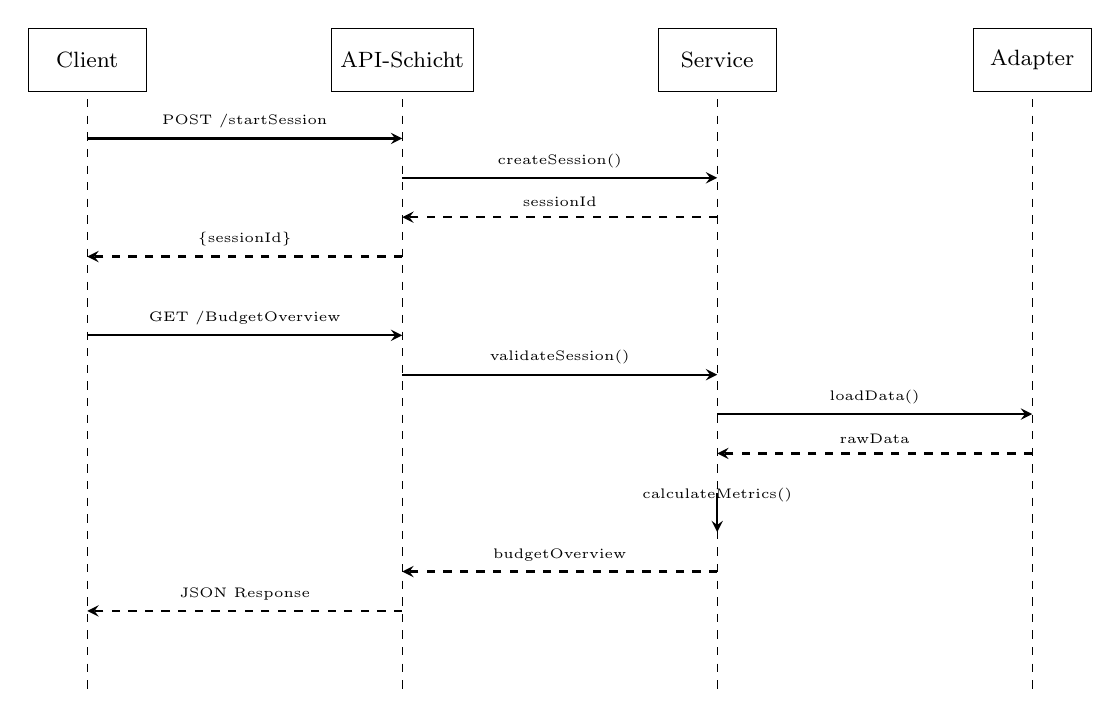
\begin{tikzpicture}[
    actor/.style={rectangle, draw, minimum width=1.5cm, minimum height=0.8cm, align=center, font=\footnotesize},
    arrow/.style={->, >=stealth, thick},
    note/.style={font=\tiny, align=left}
]
    % Akteure
    \node[actor] (client) at (0,0) {Client};
    \node[actor] (api) at (4,0) {API-Schicht};
    \node[actor] (service) at (8,0) {Service};
    \node[actor] (adapter) at (12,0) {Adapter};

    % Lebenslinien
    \draw[dashed] (0,-0.5) -- (0,-8);
    \draw[dashed] (4,-0.5) -- (4,-8);
    \draw[dashed] (8,-0.5) -- (8,-8);
    \draw[dashed] (12,-0.5) -- (12,-8);

    % Nachrichten
    \draw[arrow] (0,-1) -- node[above, font=\tiny] {POST /startSession} (4,-1);
    \draw[arrow] (4,-1.5) -- node[above, font=\tiny] {createSession()} (8,-1.5);
    \draw[arrow, dashed] (8,-2) -- node[above, font=\tiny] {sessionId} (4,-2);
    \draw[arrow, dashed] (4,-2.5) -- node[above, font=\tiny] {\{sessionId\}} (0,-2.5);

    \draw[arrow] (0,-3.5) -- node[above, font=\tiny] {GET /BudgetOverview} (4,-3.5);
    \draw[arrow] (4,-4) -- node[above, font=\tiny] {validateSession()} (8,-4);
    \draw[arrow] (8,-4.5) -- node[above, font=\tiny] {loadData()} (12,-4.5);
    \draw[arrow, dashed] (12,-5) -- node[above, font=\tiny] {rawData} (8,-5);
    \draw[arrow] (8,-5.5) -- node[above, font=\tiny] {calculateMetrics()} (8,-6);
    \draw[arrow, dashed] (8,-6.5) -- node[above, font=\tiny] {budgetOverview} (4,-6.5);
    \draw[arrow, dashed] (4,-7) -- node[above, font=\tiny] {JSON Response} (0,-7);
\end{tikzpicture}
\caption{Sequenzdiagramm: Session-Start und Datenabruf}
\label{fig:seq-session}
\end{figure}

\subsubsection{PSP-Zuordnung erstellen}

\begin{figure}[H]
\centering
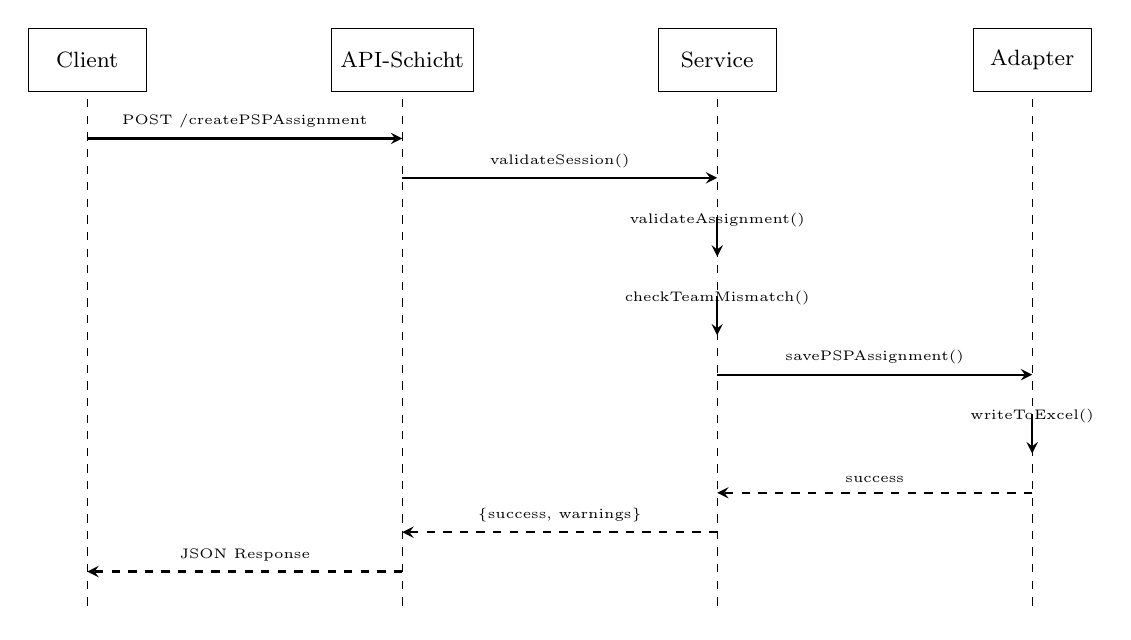
\begin{tikzpicture}[
    actor/.style={rectangle, draw, minimum width=1.5cm, minimum height=0.8cm, align=center, font=\footnotesize},
    arrow/.style={->, >=stealth, thick}
]
    % Akteure
    \node[actor] (client) at (0,0) {Client};
    \node[actor] (api) at (4,0) {API-Schicht};
    \node[actor] (service) at (8,0) {Service};
    \node[actor] (adapter) at (12,0) {Adapter};

    % Lebenslinien
    \draw[dashed] (0,-0.5) -- (0,-7);
    \draw[dashed] (4,-0.5) -- (4,-7);
    \draw[dashed] (8,-0.5) -- (8,-7);
    \draw[dashed] (12,-0.5) -- (12,-7);

    % Nachrichten
    \draw[arrow] (0,-1) -- node[above, font=\tiny] {POST /createPSPAssignment} (4,-1);
    \draw[arrow] (4,-1.5) -- node[above, font=\tiny] {validateSession()} (8,-1.5);
    \draw[arrow] (8,-2) -- node[above, font=\tiny] {validateAssignment()} (8,-2.5);
    \draw[arrow] (8,-3) -- node[above, font=\tiny] {checkTeamMismatch()} (8,-3.5);
    \draw[arrow] (8,-4) -- node[above, font=\tiny] {savePSPAssignment()} (12,-4);
    \draw[arrow] (12,-4.5) -- node[above, font=\tiny] {writeToExcel()} (12,-5);
    \draw[arrow, dashed] (12,-5.5) -- node[above, font=\tiny] {success} (8,-5.5);
    \draw[arrow, dashed] (8,-6) -- node[above, font=\tiny] {\{success, warnings\}} (4,-6);
    \draw[arrow, dashed] (4,-6.5) -- node[above, font=\tiny] {JSON Response} (0,-6.5);
\end{tikzpicture}
\caption{Sequenzdiagramm: PSP-Zuordnung erstellen}
\label{fig:seq-assignment}
\end{figure}

\subsection{Designentscheidungen}

Im Folgenden werden zentrale Designentscheidungen dokumentiert und begründet \citep{bass2021}.

\subsubsection{DE-01: Keine Datenbank}

\textbf{Entscheidung}: Die Middleware verwendet keine eigene Datenbank, sondern liest Daten bei jedem Request direkt aus der Excel-Datei.

\textbf{Begründung}: Excel bleibt als \enquote{Single Source of Truth} erhalten, wodurch keine Synchronisationsprobleme zwischen einer Datenbank und Excel entstehen. Zudem vereinfacht sich das Deployment, da keine DB-Bindung auf der BTP erforderlich ist, und die Konsistenz mit dem bestehenden Workflow der Anwender bleibt gewahrt.

\textbf{Trade-off}: Höhere Latenz bei jedem Request, da Excel geparst werden muss. Für die erwartete Nutzerzahl (< 50 gleichzeitig) akzeptabel.

\subsubsection{DE-02: Session-Management im RAM}

\textbf{Entscheidung}: Sessions werden im Arbeitsspeicher des Servers gehalten, nicht persistiert.

\textbf{Begründung}: Die Implementierung ist einfach, es wird keine zusätzliche Infrastruktur wie Redis oder eine Datenbank benötigt, und Sessions sind kurzlebig (Arbeitstag).

\textbf{Trade-off}: Bei Server-Neustart gehen Sessions verloren. Benutzer müssen sich neu einloggen. Dieses Problem ist in verteilten Systemen bekannt und kann durch externe Session-Speicher wie Redis gelöst werden \citep{tanenbaum2017, richardson2018}. Für einen Prototyp ist die In-Memory-Lösung akzeptabel.

\subsubsection{DE-03: OData statt GraphQL}

\textbf{Entscheidung}: Die API wird als OData v4 Service implementiert, nicht als GraphQL.

\textbf{Begründung}: Das SAP-Ökosystem ist auf OData ausgerichtet und SAP Fiori erwartet OData-Services. SAP CAP generiert OData automatisch aus CDS-Definitionen, sodass keine zusätzlichen Abhängigkeiten entstehen.

\textbf{Trade-off}: GraphQL bietet zwar flexiblere Abfragemöglichkeiten und reduziert Over-/Underfetching \citep{brito2019}, jedoch überwiegen im SAP-Kontext die Vorteile der nativen OData-Unterstützung. Studien zeigen, dass die Migration zu GraphQL erheblichen Aufwand erfordert, während OData im Enterprise-Umfeld etabliert ist \citep{vogel2018}.

\subsubsection{DE-04: Adapter-Pattern statt Strategy-Pattern}

\textbf{Entscheidung}: Das Adapter-Pattern wird zur Abstraktion der Datenquellen verwendet.

\textbf{Begründung}: Der Adapter übersetzt zwischen inkompatiblen Schnittstellen (Excel und OData) und hat eine klare Verantwortlichkeit: die Transformation von der spezifischen Datenquelle in ein einheitliches Modell. Das Strategy-Pattern wäre hingegen bei austauschbaren Algorithmen passender und adressiert eine andere Problemstellung \citep{gamma1994}.

\subsection{Fehlerbehandlung}

Die Middleware implementiert eine einheitliche Fehlerbehandlung für alle API-Endpunkte:

\begin{table}[H]
\centering
\caption{HTTP-Statuscodes und Fehlerszenarien}
\label{tab:error-handling}
\begin{tabularx}{\textwidth}{cl>{\raggedright\arraybackslash}X}
\toprule
\textbf{Code} & \textbf{Bedeutung} & \textbf{Szenario} \\
\midrule
200 & OK & Erfolgreiche Anfrage (inkl. PSP-Zuordnung erstellt) \\
400 & Bad Request & Ungültige Parameter (z.B. fehlende User Story) \\
401 & Unauthorized & Keine oder ungültige Session-ID \\
404 & Not Found & Projekt oder Ressource existiert nicht \\
409 & Conflict & PSP-Zuordnung existiert bereits \\
500 & Server Error & Excel-Datei nicht lesbar, interner Fehler \\
\bottomrule
\end{tabularx}
\end{table}

Fehler werden als JSON-Objekt mit \texttt{error}-Feld zurückgegeben:

\begin{lstlisting}[caption={Fehler-Response Format}, label={lst:error-response}]
{
    "error": {
        "code": "NO_SESSION",
        "message": "Keine aktive Session. Bitte zuerst startSession aufrufen.",
        "target": "x-session-id"
    }
}
\end{lstlisting}
